%%
%% This is file `sample-authordraft.tex',
%% generated with the docstrip utility.
%%
%% The original source files were:
%%
%% samples.dtx  (with options: `authordraft')
%% 
%% IMPORTANT NOTICE:
%% 
%% For the copyright see the source file.
%% 
%% Any modified versions of this file must be renamed
%% with new filenames distinct from sample-authordraft.tex.
%% 
%% For distribution of the original source see the terms
%% for copying and modification in the file samples.dtx.
%% 
%% This generated file may be distributed as long as the
%% original source files, as listed above, are part of the
%% same distribution. (The sources need not necessarily be
%% in the same archive or directory.)
%%
%% The first command in your LaTeX source must be the \documentclass command.
\documentclass[sigplan,screen]{acmart}
\graphicspath{ {./images/} }

\usepackage{caption}
\usepackage{subcaption}
\usepackage{indentfirst}


%% NOTE that a single column version may required for 
%% submission and peer review. This can be done by changing
%% the \doucmentclass[...]{acmart} in this template to 
%% \documentclass[manuscript,screen]{acmart}
%% 
%% To ensure 100% compatibility, please check the white list of
%% approved LaTeX packages to be used with the Master Article Template at
%% https://www.acm.org/publications/taps/whitelist-of-latex-packages 
%% before creating your document. The white list page provides 
%% information on how to submit additional LaTeX packages for 
%% review and adoption.
%% Fonts used in the template cannot be substituted; margin 
%% adjustments are not allowed.

%%
%% \BibTeX command to typeset BibTeX logo in the docs
\AtBeginDocument{%
  \providecommand\BibTeX{{%
    \normalfont B\kern-0.5em{\scshape i\kern-0.25em b}\kern-0.8em\TeX}}}

%% Rights management information.  This information is sent to you
%% when you complete the rights form.  These commands have SAMPLE
%% values in them; it is your responsibility as an author to replace
%% the commands and values with those provided to you when you
%% complete the rights form.

%% These commands are for a PROCEEDINGS abstract or paper.
\acmConference[PRI 21/22]{Building an Information Search System}{November 16, 2021}{Porto, PT}
\acmBooktitle{Building an Information Search System,
  November 16, 2021, Porto, PT}


%%
%% Submission ID.
%% Use this when submitting an article to a sponsored event. You'll
%% receive a unique submission ID from the organizers
%% of the event, and this ID should be used as the parameter to this command.
%%\acmSubmissionID{123-A56-BU3}

%%
%% The majority of ACM publications use numbered citations and
%% references.  The command \citestyle{authoryear} switches to the
%% "author year" style.
%%
%% If you are preparing content for an event
%% sponsored by ACM SIGGRAPH, you must use the "author year" style of
%% citations and references.
%% Uncommenting
%% the next command will enable that style.
%%\citestyle{acmauthoryear}

\settopmatter{printacmref=false} % Removes citation information below abstract
\renewcommand\footnotetextcopyrightpermission[1]{} % removes footnote with conference information in first column
\pagestyle{plain} % removes running headers


%%
%% end of the preamble, start of the body of the document source.
\begin{document}

%%
%% The "title" command has an optional parameter,
%% allowing the author to define a "short title" to be used in page headers.
\title{% 
    Building an Information Search System \\
    \large Information Processing and Retrieval Project
    }


%%
%% The "author" command and its associated commands are used to define
%% the authors and their affiliations.
%% Of note is the shared affiliation of the first two authors, and the
%% "authornote" and "authornotemark" commands
%% used to denote shared contribution to the research.
\author{Paulo Ribeiro}
\email{up201806505@edu.fe.up.pt}
\affiliation{%
  \institution{Faculdade de Engenharia da Universidade do Porto}
  \streetaddress{Rua Doutor Roberto Frias s/n}
  \city{Porto}
  \country{Portugal}
  \postcode{4200-465}
}

\author{Pedro Ferreira}
\email{up201806506@edu.fe.up.pt}
\affiliation{%
  \institution{Faculdade de Engenharia da Universidade do Porto}
  \streetaddress{Rua Doutor Roberto Frias s/n}
  \city{Porto}
  \country{Portugal}
  \postcode{4200-465}  
}

\author{Pedro Ponte}
\email{up201809694@edu.fe.up.pt}
\affiliation{%
 \institution{Faculdade de Engenharia da Universidade do Porto}
 \streetaddress{Rua Doutor Roberto Frias s/n}
 \city{Porto}
 \country{Portugal}
 \postcode{4200-465}
 }

%%
%% The abstract is a short summary of the work to be presented in the
%% article.
\begin{abstract}
  This report pretends to detail the implementation of an information search system for the curricular unit \textbf{Information Processing and Retrieval}, for the  Master in Informatics and Computing Engineering. This implementation was divided into three milestones, relative to data collection and preparation, information querying and retrieval, and retrieval evaluation.
\end{abstract}

%%
%% Keywords. The author(s) should pick words that accurately describe
%% the work being presented. Separate the keywords with commas.
\keywords{datasets, data processing, information retrieval, retrieval evaluation, information search system}

%% A "teaser" image appears between the author and affiliation
%% information and the body of the document, and typically spans the
%% page.
\begin{teaserfigure}
    \begin{center}
      \includegraphics[scale = 0.6]{samples/feup.png}
      \Description{Faculdade de Engenharia da Universidade do Porto logo}
      \label{fig:teaser}
    \end{center}
\end{teaserfigure}

%%
%% This command processes the author and affiliation and title
%% information and builds the first part of the formatted document.
\maketitle

\section{Introduction}

The goals of the first milestone of this project are to correctly prepare the data for the information retrieval tool to be implemented in the second milestone. The first step is to explore different datasets and choose a captivating one. After being familiar with its data, the next step is to think of a possible data processing pipeline, adequate for our problem.

Upon defining this pipeline, some essential steps are necessary, such as assessing the data quality by looking for missing or invalid values and handling them, besides fixing some other minor problems. In our case, data extraction was also applied to fill or update missing values. A step focused on data exploration is also required, with the gathering of some important statistics and the creation of distinct plots representing the data involved.

\section{Milestone 1 - Data Preparation}

\subsection{Data Collection}

For this step, our first move was choosing an interesting collection of data. This meant picking a dataset with a somewhat large amount of information that would be useful and relevant for the given purpose.

While seeking a dataset worthy of fitting the requirements, various options that ended up not being worked upon came across. Datasets related to videogames, as a gathering of all players present in the EA sports franchise FIFA or club and sportsman data from SEGA game Football Manager, were some considered examples. The digital distribution service Steam, from Valve corporation, was also taken into account. Although these datasets were able to fill almost all the requirements needed, the lack of sizeable texts of individual information could be a non so good aspect that would limit us in the future.

So, the final choice ended up related to the topic of Netflix's TVSeries and movies. Two different datasets about this topic were found. The choice on which one to go with was based on the existence of a vaster number of relevant parameters and the presence of a summary column that would be useful for full-text searches needed for future work.

The information was also gathered from the IMDb website. This would facilitate the search for missing intel and bring confidence to the work while using a trustworthy source for the data collected since IMDb is a well-known and prestigious platform for online TV series and films.

The dataset chosen has information in the form of the following columns:

\begin{itemize}
\item {\textit{imdb\_id}}: Show id from the IMDb website;
\item {\textit{title}}: The title of the show;
\item {\textit{popular\_rank}}: The popular rank of the show;
\item {\textit{certificate}}: The age restrinction of a show;
\item {\textit{startYear}}: Release year of a show;
\item {\textit{endYear}}: Year the show ended;
\item {\textit{episodes}}: Number of episodes of a show;
\item {\textit{runtime}}: Mean time duration of a show;
\item {\textit{type}}: Type of a show;
\item {\textit{orign\_country}}: Origin country of the show;
\item {\textit{title}}: The title of the show;
\item {\textit{language}}: The language a show was produced on;
\item {\textit{summary}}: Summary of the show;
\item {\textit{rating}}: IMDb rating of the show;
\item {\textit{numVotes}}: Number of votes for show rating;
\item {\textit{genres}}: Genres categories of a show;
\item {\textit{isAdult}}: Presence of adult content in the show;
\item {\textit{cast}}: Cast of the show;
\item {\textit{image\_url}}: Poster of the show.
\end{itemize}

\subsection{Pipeline Design}

After deciding which dataset to explore, our next step is to define a concise pipeline for the data processing, so that we structure its steps in the most adequate way to our problem. We started by documenting it using a diagram to better visualize the data flow. This diagram is shown in the following figure:

\begin{figure}[h]
  \centering
  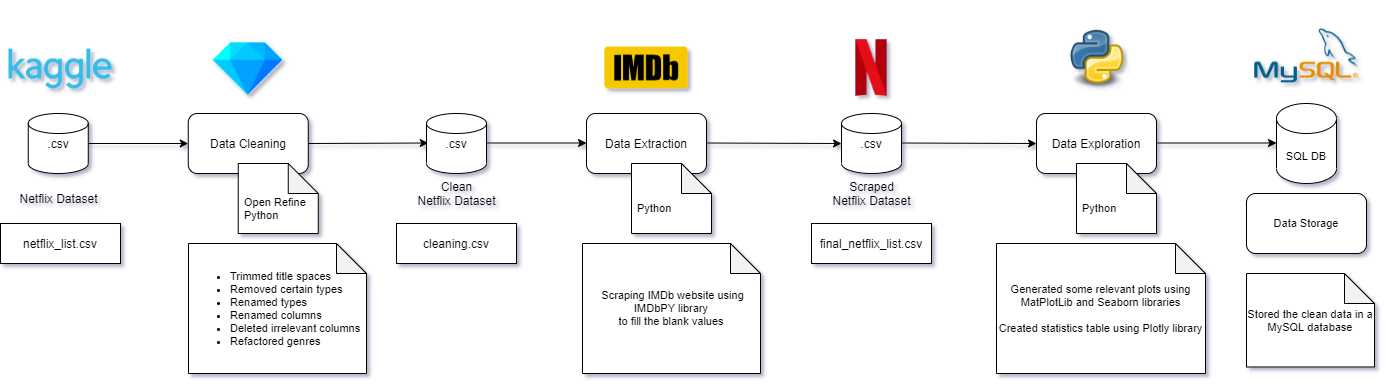
\includegraphics[width=\linewidth]{samples/Pipeline.png}
  \caption{Data processing pipeline}
  \Description{Data processing pipeline diagram}
\end{figure}

The starting point of our pipeline consists of the Netflix dataset, which we retrieved from Kaggle, in a CSV format. 

Then, our first step is to clean this data by fixing some issues and adapting it to our best interest. This includes removing some irrelevant columns from our dataset, renaming others and refactoring some data formats to make them more easily accessible. The previous step results in a clean CSV file, where these changes are already applied. 

After this, we thought it was interesting to fill the missing values of the dataset with recent information gathered from the web. The indicated step is called Data Extraction. It was decided to resort to the IMDb website and apply some scraping to complete the information about the shows since it is the world's most popular and authoritative source for this type of content. The fact that the original dataset was built retrieving information from this same source also helped in the decision. Since we desired a consistent dataset, the newly collected data shouldn't be too different from the existing one.

The aforementioned process results in the last CSV file, from which it can now be performed the Data Exploration step, where we gather some important statistics of our problem and generate some relevant plots to better illustrate some of its characteristics. 

Finally, our last step is to store the data in a way that its access becomes easy and efficient. For this, we decided to use a MySQL database. After all these steps, the data is now ready to be retrieved every time it is needed.

\subsection{Data Cleaning}

Initially, we have a dataset with 7008 rows and 19 columns. Some of the columns contain irrelevant information, others have repeated data and some of them contain similar categories that could be joined together.

In our analysis on \textit{OpenRefine}, we conclude that the column \textit{isAdult} adds no value to our dataset, since it has all values as '0', thus we removed it. We also checked that the columns \textit{plot} and \textit{summary} are very similar, but the \textit{summary} has more information than \textit{plot}, so we opted to delete the \textit{plot} column.

Then, we noticed there were some pairs of repeated titles, although one has a leading whitespace whereas the other doesn't. We found out that the ones with no initial space represent a 'tvSeries' and the others were a 'tvEpisode'. After some search on IMDb platform using the \textit{imdbID}, it was concluded the 'tvEpisodes' are, in reality, episodes of the 'tvSerie' with the same name, so we opted to delete all the rows that have 'tvEpisode' as \textit{type}.

Continuing \textit{type} analysis, the dataset only has one entry with 'videogame'. Since we consider that only having  one value of this type doesn't add any value to our future search system, we decided to drop this entry. There are also two rows that, in addition to having a null \textit{type}, do not have other several values defined, so they were also taken off. After removing these types, we still have: 'tvSeries', 'tvMiniSeries', 'tvShort', 'tvSpecial', 'tvMovie', 'video', 'movie', 'short'. We decided to rename 'tvSeries' for 'series', 'tvMiniSeries' for 'miniSeries', 'tvShort' for 'short', 'tvSpecial' for 'special', 'tvMovie' for 'movie' and 'video' for 'animation'.

Finally, it was decided to rename some of the columns in order to have them all in \textit{lowerCamelCase} style and, for each \textit{genres} column entry, put all its values inside an array.  

Finished the cleaning step, we have a dataset with 6216 rows and 17 columns.

\subsection{Data Extraction}

Once the data cleaning process is finished, we proceed to an attempt to fill in the missing values.

To do this, we used Python and a library called IMDbPY. With this library, we can get almost all types of information about the IMDb shows.

In the case of \textit{certificate} column, initially we had only a certificate for each show, but the country to which the certificate applies was not always the same. Taking this into account, we decided to extract from IMDb all the certificates that apply to each show and store them into a dictionary converted into string, in the format of \textit{country : certificate}.

To try to complete some of the missing values in \textit{startYear} and \textit{endYear} columns, we filled all the shows that are missing both values simultaneously and all the series or miniSeries that don't have the \textit{endYear} value.

To complete the null values in \textit{episodes} column, we have scraped from IMDb the number of episodes of each series or miniSeries that are missing this value.

For \textit{runtime}, \textit{originCountry}, \textit{language}, \textit{summary}, \textit{rating}, \textit{numVotes}, \textit{genres} and \textit{cast} columns, we try to extract from IMDb the missing values of these dataset parameters.

\subsection{Data Exploration}

Now that our data is finally clean and complete, we are ready to start exploring all its 6216 entries. In this step, we generate some relevant graphics so that we can better visualize our information domain and possibly deduce some conclusions. We used Python to achieve these results, namely the \textbf{MatPlotLib} and \textbf{Seaborn} libraries to generate the charts and the library \textbf{Plotly} to create a statistics table.

Our first thought was to get an overview of one of the most important attributes of our dataset: the type of the show. We decided that a Bar Chart was the most suited approach to see the dimensions of each of those types. The graphic is shown in the next figure: 

\begin{figure}[h]
  \centering
  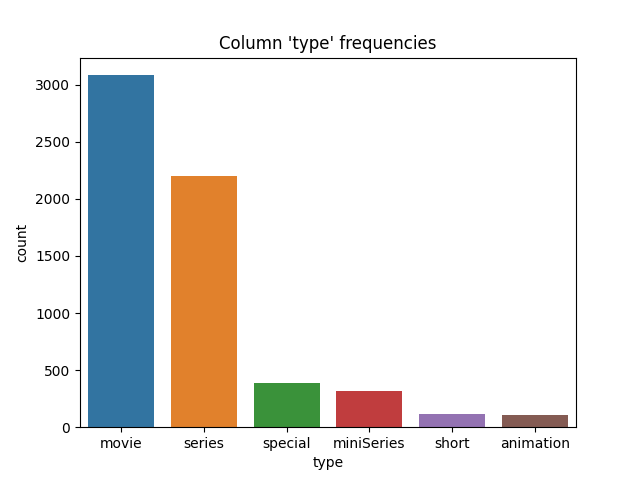
\includegraphics[width=\linewidth, height = 35mm]{samples/typeFrequencies.png}
  \caption{'Type' Bar Chart}
  \Description{'Type' Bar Chart}
\end{figure}

As we can see, the dataset is especially filled with movies and series, followed by some less frequent types, such as specials, mini-series, shorts and animations.

Then, we thought it was interesting to study the evolution of the ratings over the decades. For this, we decided to use a Box Plot, since it gives us the most information about that distribution, namely the ranges, outliers and quartiles. Before generating the graphic, we first had to group the years by decades, exclude the "Not available" values and sort the decades. That resulted in this figure:

\newpage

\begin{figure}[h]
  \centering
  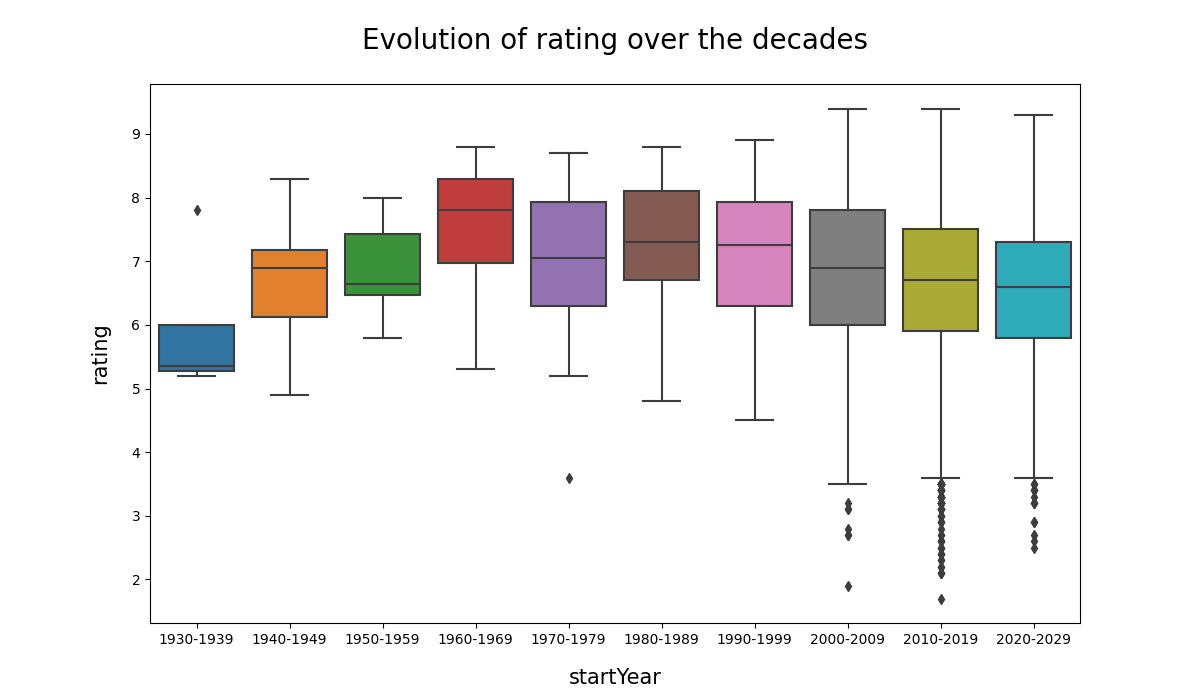
\includegraphics[width=\linewidth]{samples/ratingEvolution.png}
  \caption{'Rating' Box Plot}
  \Description{'Rating' Box Plot}
\end{figure}

The number of shows from recent decades is naturally higher than the number of older shows. As a consequence, the rating range of the recent decades is larger. Both the minimum and maximum of the ratings were achieved in the $21^{\text{st}}$ century. The mean of the ratings has also been slightly decreasing throughout the years. It's also possible to notice some outliers, marked by the dots.

Next, we wanted to see the distribution of the languages and origin countries. We knew there were too many distinct values in these columns to represent them all in a single diagram. Thus, the best and cleaner way we found to solve this problem was to create a Pie Chart, where we would call one of the divisions "Others". This chart should show the nine most common languages/origin countries and the \emph{Others} division would encompass all the less frequent ones. Both of these charts can be seen in the following figures:

\begin{figure}[h]
  \centering
  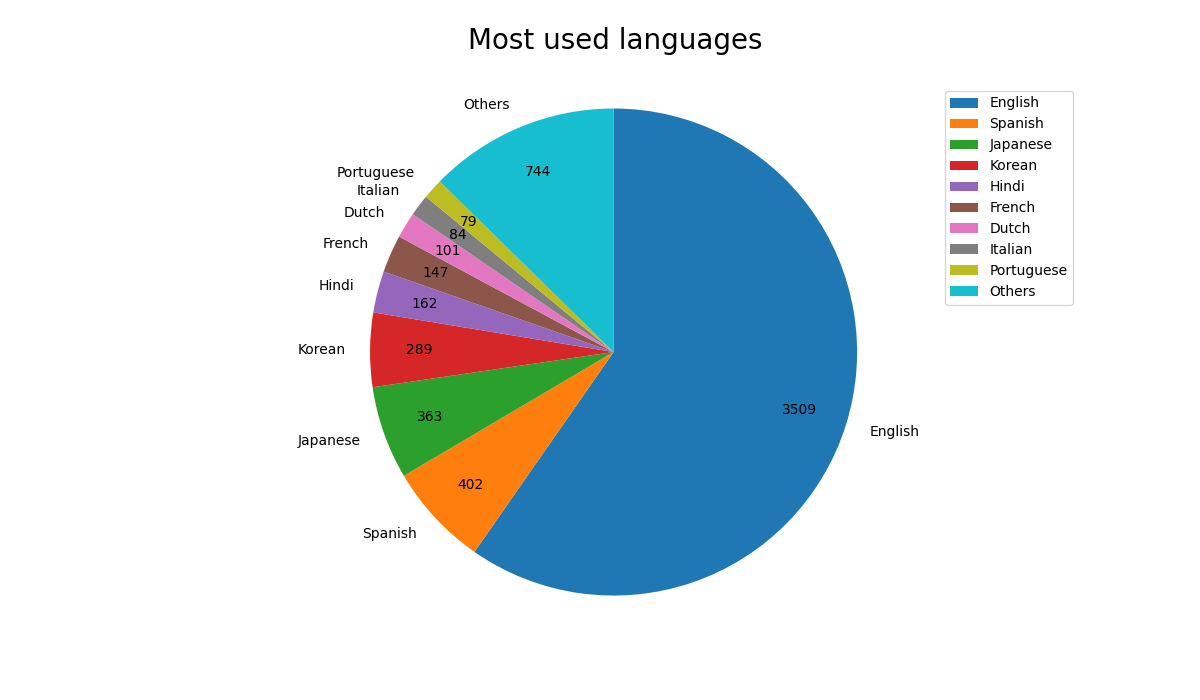
\includegraphics[width=\linewidth]{samples/languagesDistribution.png}
  \caption{'Language' Distribution Pie Chart}
  \Description{'Language' Distribution Pie Chart}
\end{figure}

\begin{figure}[h]
  \centering
  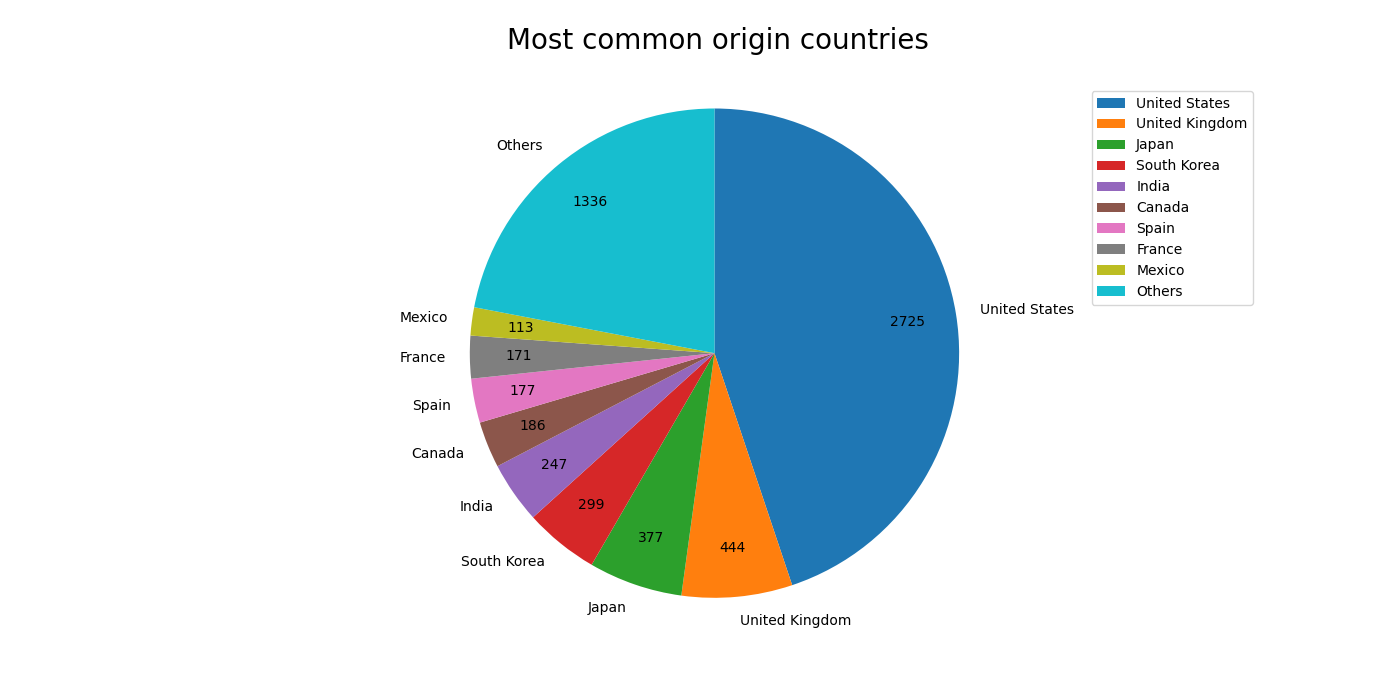
\includegraphics[width=\linewidth]{samples/countriesDistribution.png}
  \caption{'Countries' Distribution Pie Chart}
  \Description{'Countries' Distribution Pie Chart}
\end{figure}

\newpage

We also thought it was interesting to show the distribution of the genres. This was a more challenging quest since each show can have many genres associated. So we had to create and fill a dictionary where for each genre there is a count associated, with the number of times that genre is present in a show. Then, we generated a Bar Chart with the nine most common genres and the \emph{Others} column encompassing the less frequent ones, which is shown in the following figure:

\begin{figure}[h]
  \centering
  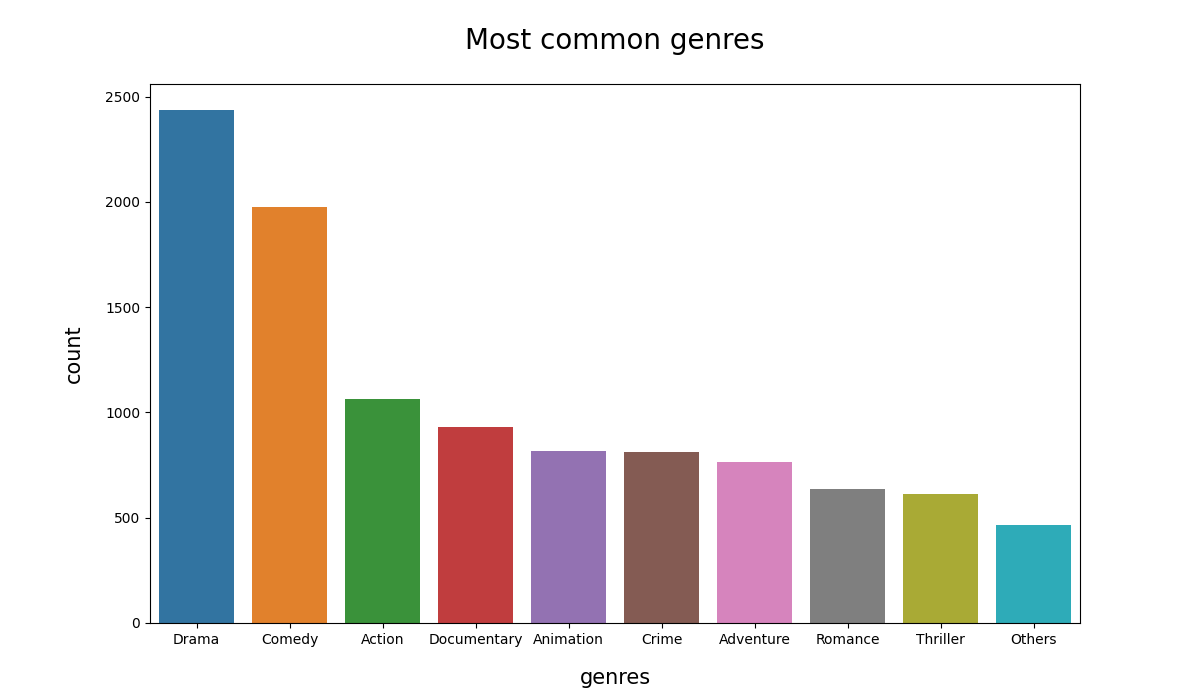
\includegraphics[width=\linewidth, height = 35mm]{samples/genresDistribution.png}
  \caption{'Genre' Bar Chart}
  \Description{'Genre' Bar Chart}
\end{figure}

Similarly, it would be relevant to know the actors with the most appearances in our dataset. The same strategy of the genre chart was applied, and we got a dictionary containing every actor and their number of appearances. After this, we generated the chart with the top 20 of the actors with the most participations, which can be seen in the next figure:

\begin{figure}[h]
  \centering
  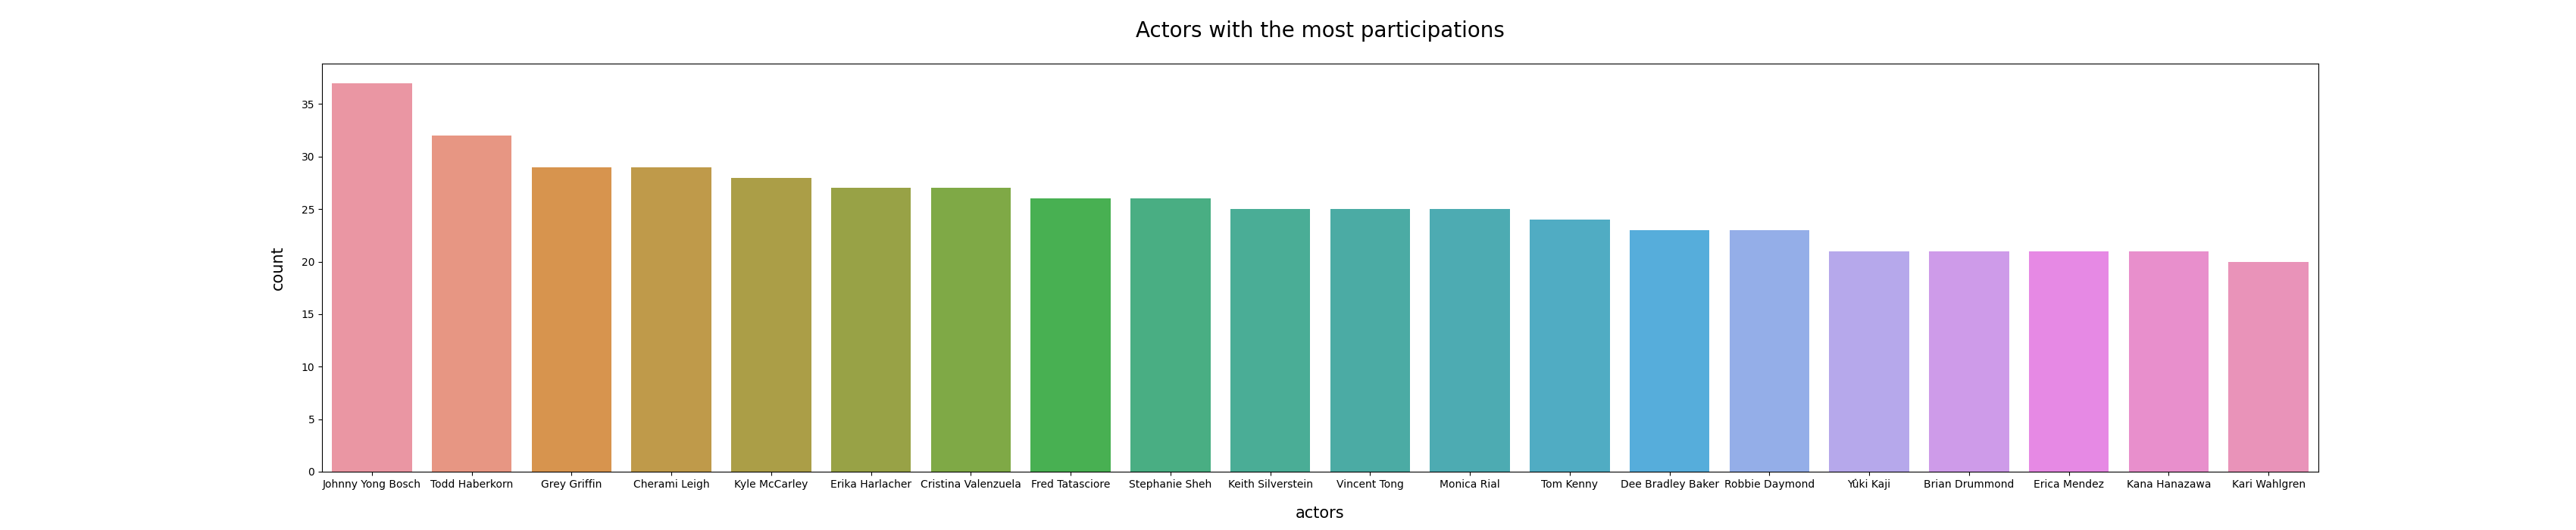
\includegraphics[width=\linewidth]{samples/castDistribution.png}
  \caption{'Cast' Bar Chart}
  \Description{'Cast' Bar Chart}
\end{figure}

Finally, we wanted to know some basic statistics of our dataset, such as the means of the runtimes of each show type and the total number of distinct values of some columns, which we gathered in a table, shown in the following figure:
\newpage

\begin{figure}[h]
  \centering
  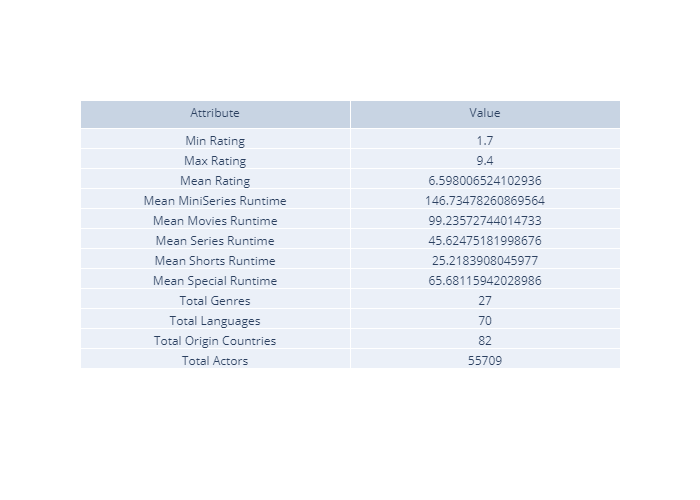
\includegraphics[width=\linewidth, height = 33mm]{samples/statisticsTable.png}
  \caption{Basic statistics of the dataset}
  \Description{Basic statistics of the dataset}
\end{figure}

\subsection{UML Design}

\begin{figure}[h]
  \centering
  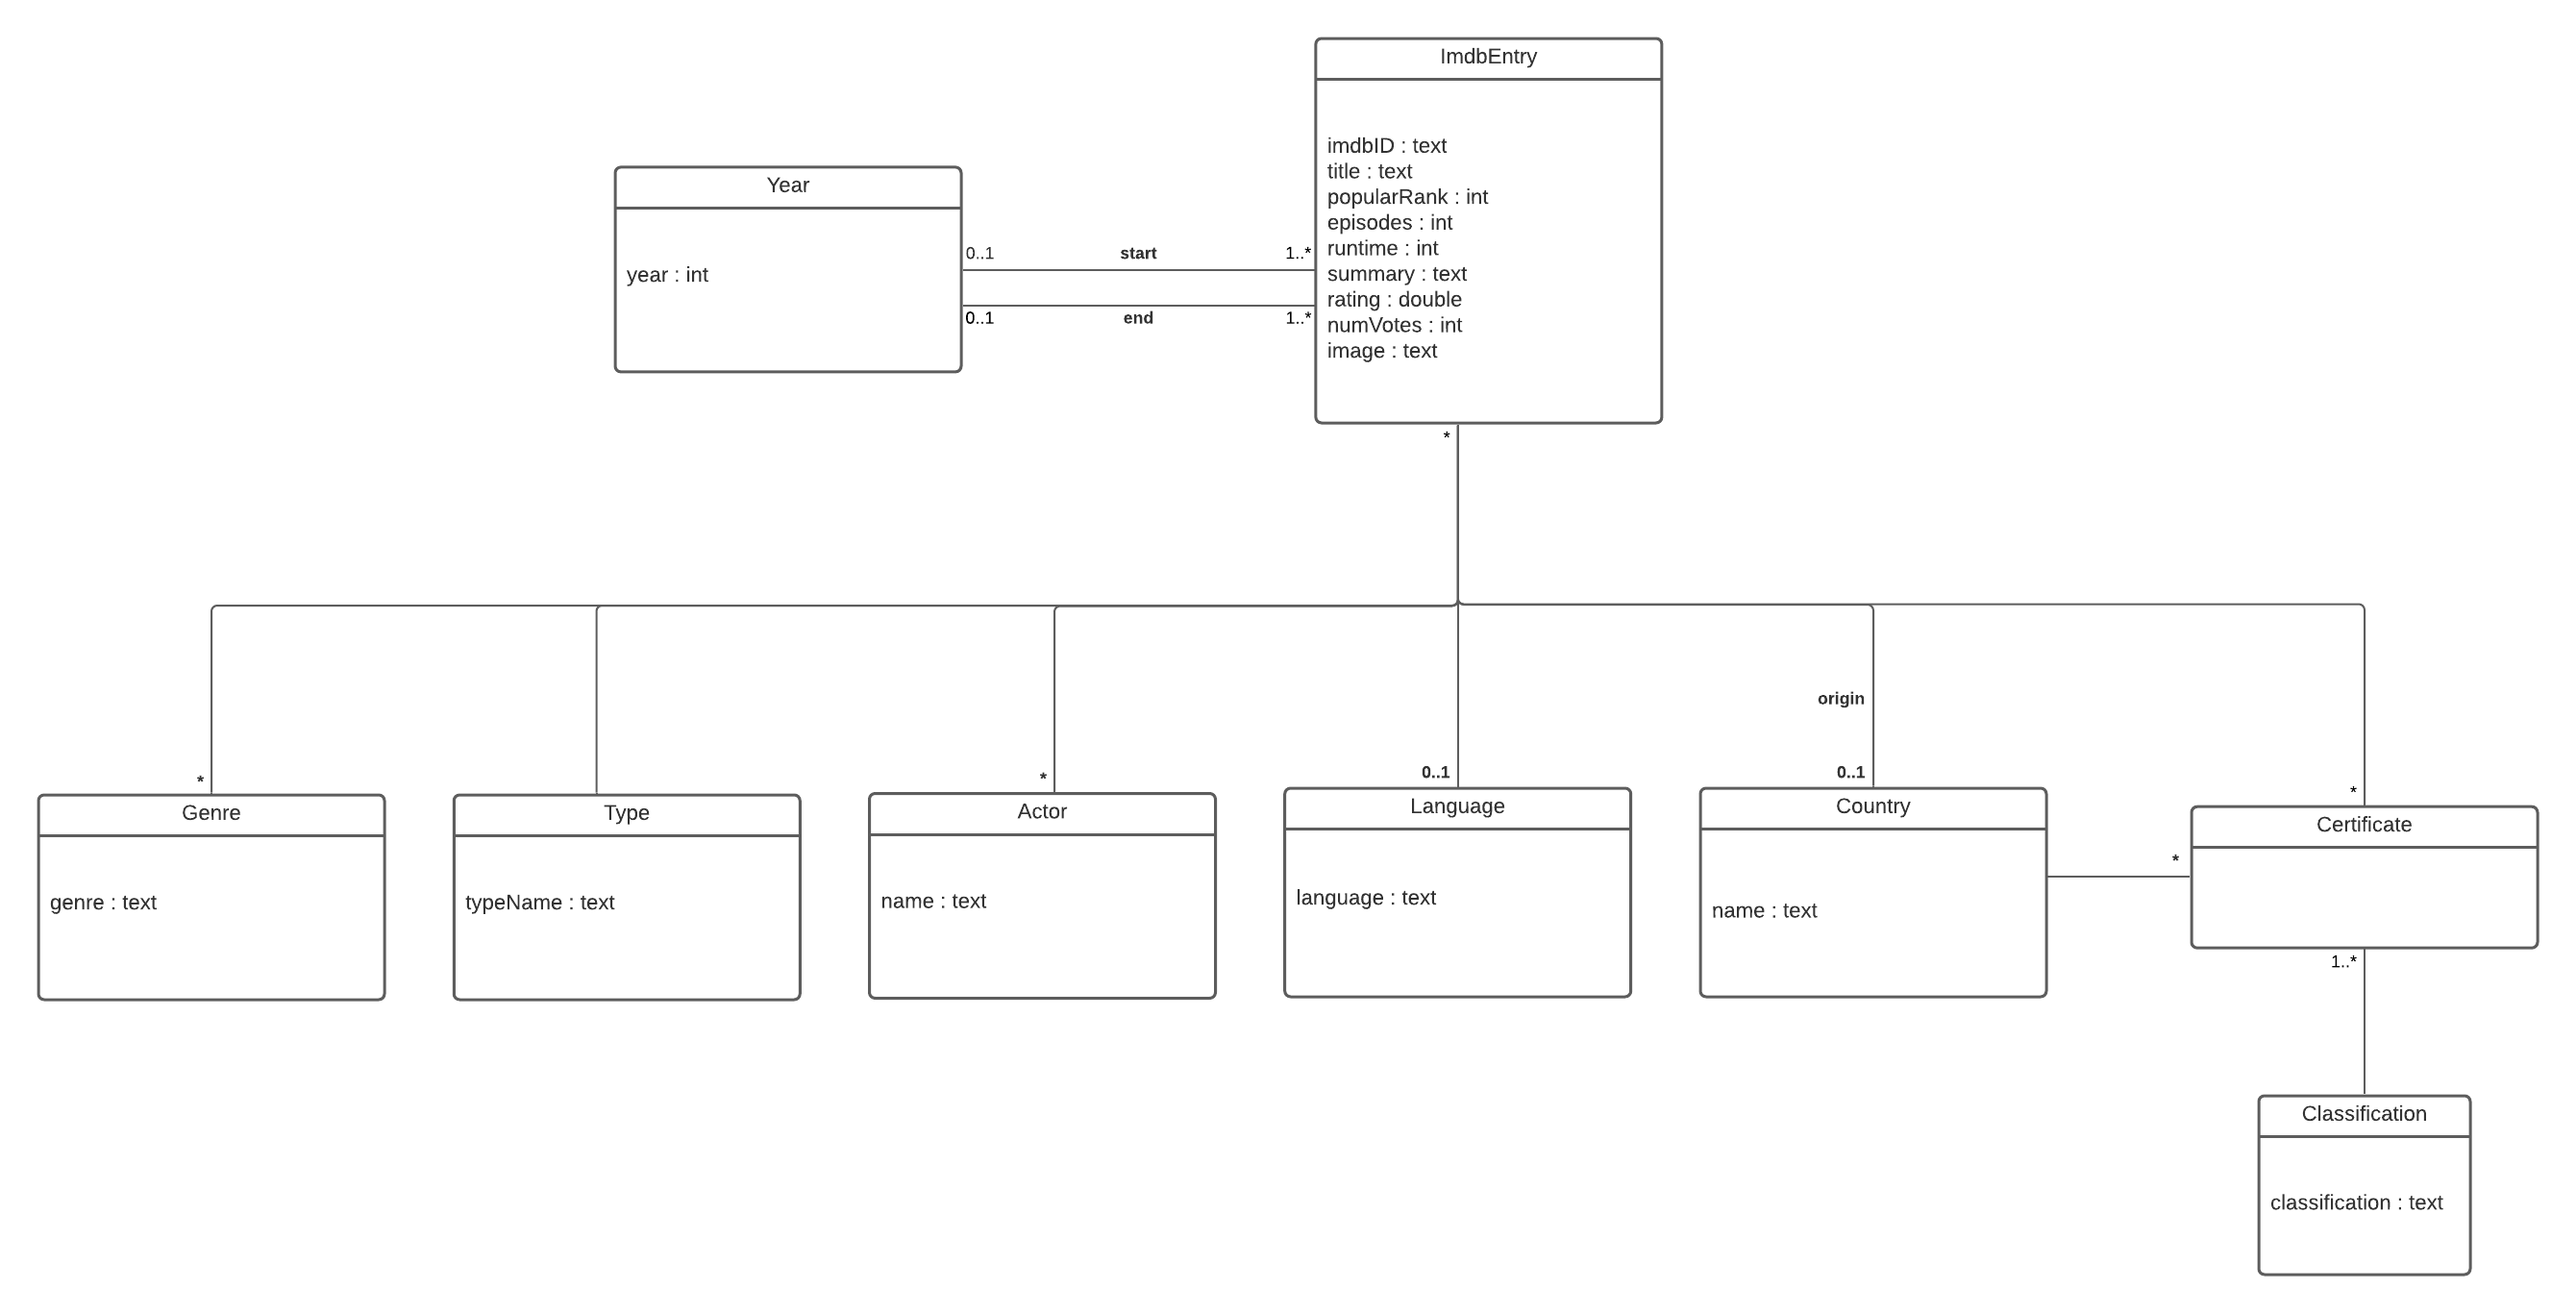
\includegraphics[width=\linewidth]{samples/UML.png}
  \caption{UML diagram for database creation}
  \Description{UML diagram representation}
\end{figure}

To be able to create a database that could support saving all the information in a useful and efficient way, a UML was carefully thought and created.

The main class ImdbEntry was created to represent each show. This class is composed by a parameter imdbID, title, popularRank, episodes, runtime, rating, summary, numVote and image.

As there are two columns dedicated to years on our dataset and repeated values for many shows, a new class Year was created having two different relations with ImdbEntry (one for the startYear and the other for the endYear).

Furthermore, five new classes were created since the same issue as in the year appeared, where the values would be very repetitive. This way, a class genre (with the genres a show can have), type (class with the various types a show can be, whether it is a tv series, film, etc), actor (class with the name of an actor that can participate in a show), language (languages a show can be originally made on) and country (countries where the show can be taken place) were created.

Finally, a new class Certificate was created, as well as a connection to the ImdbEntry. This object also has a connection to the country class and to a new classification class that will give the actual value for the certification. This new class classification will depend on the country correspondent. This happens because different countries classify their shows on different scales and will be useful in future work, allowing us to get search results in all the different classifications.


\end{document}
\endinput
%%
%% End of file `sample-authordraft.tex'.
